\chapter{System call based detection}
\label{chap:syscalltheory}
In this chapter, we will discuss the overall strategy of our second approach for malware detection, which uses system call [explanation] traces of applications to predict malicious activity. Following chapters will discuss the implementation details of this model and also the results achieved in our experiment using this model.\\

The central idea is to run an application for a specific amount of time (in our simulation - 10 seconds). During its execution, the details about the system calls it make to the operating system are recorded. We developed a machine learning model/classifier that can detect malware based on its system call trace. The syscall records of known malwares and known non-malwares are used to train the classifier. There will be two phases: training and classification. How the known malware and non-malware traces will be used to train the classifier is described in section ~\ref{sec:syscalltheorytrain}. Section ~\ref{sec:syscalltheoryclassify} decribes how the model will classify an unknown app using its syscall trace. 

\section{Training}
\label{sec:syscalltheorytrain}
We will use a set of applications consisting both known malwares and known non-malwares as the training dataset. We will collect system call traces of all applications of the training dataset (all of the applications will be run for a specific amount of time). The system call trace of a single application is a list of system calls the application used during execution. For example: \textbf{\{recv, semget, msgget, \ldots \}}; where \textbf{recv}, \textbf{semget}, \textbf{msgget} are system calls.

After collecting system call traces, We aggregate this traces to create two binary relation matrices $M_{mal}$ and $M_{nmal}$. $M_{mal}$ shows relation between system calls and malware applications, Where $M_{nmal}$ shows relationship between system calls and non-malwares. $M_{mal}$ and $M_{nmal}$ matrices are defined as follows:\\
\[ M_{mal}(i,j) =
  \begin{cases}
      1       & \quad \text{if } i^{th} \text{ malware uses } j^{th} \text{ syscall}\\
      0       & \quad \text{otherwise}\\
  \end{cases}
\]\\
\[ M_{nmal}(i,j) =
  \begin{cases}
      1       & \quad \text{if } i^{th} \text{ non-malware uses } j^{th} \text{ syscall}\\
      0       & \quad \text{otherwise}\\
  \end{cases}
\]
\\\\
Then we calculate the Goodness Rating of $j^{th}$ syscall, $G_j$ as follows,
\[
G_j = \frac{1}{N_{nmal}}\sum_{i=1}^{N_{nmal}} M_{nmal}(i,j) - \frac{1}{N_{mal}}\sum_{i=1}^{N_{mal}} M_{mal}(i,j)
\]
where $N_{nmal}$ and $N_{mal}$ are number of non-malware and malware samples.
\\
\section{Classification}
\label{sec:syscalltheoryclassify}
To classify an unknown application as \emph{malware} or \emph{non-malware}, first, we execute the application for the same time duration duration we used with each training application. We collect the system call trace of that application during that execution, same as before. But this time, we also record the frequency of each syscall used by the application during execution. So now, the syscall trace of an application during classification phase can be expressed as a list of pairs of syscalls and their frequencies. For example: \textbf{\{(recv,1032), (semget, 143), \ldots \}} is a trace of an application which called the \textbf{recv} routine 1032 times, \textbf{semget} 143 times and so on.

Then we define the Goodness Rating of that application as follows
\[
G_{app} = \sum_{s \in S_{app}} G_s \times F_s
\]

Where, $S_{app}$ is the set of system calls used by $app$ and $F_s$ is the frequency of syscall $s$ in $app$.

If we assume that malwares uses similar system calls which are distinctive from those used by non-malwares; It is logical to assume that a malware will use more syscalls those has lower goodness ratings and less syscalls having higher goodness ratings. The opposite can be said for non-malware applications. So this will result in higher goodness ratings of non-malware applications and lower goodness rating for malware applications.

Now for classification, we check if the goodness rating of the application under inspection exceeds some threshold. If so, we classify it as non-malware. otherwise we flag it as malware. 
\[
\begin{cases}
      \text{app is a malware}  & \quad \text{if } G_{app} > T\\
      \text{app is not a malware} & \quad \text{otherwise}\\
  \end{cases}
\]

Where, $T$ is a threshold. Theoretically, the threshold should be zero. But it actually depends on the experiment and the training data used. We will classify apps in validation dataset and calculate some metrics to evaluate our model. We will calculate the following metrics:

\begin{enumerate}
\item \textbf{Accuracy}
\[
    ACC = \frac{TP + TN}{P + N}
\]
\item \textbf{Sensitivity}/\textbf{Recall}  or \textbf{True Positive Rate}
\[
    TPR = \frac{TP}{P}
\]
\item \textbf{Specificity} or \textbf{True Negative Rate}
\[
    SPC = \frac{TN}{N}
\]
\item \textbf{Precision} or \textbf{Positive Predictive Value}
\[
    PPV = \frac{TP}{TP + FP}
\]
\item \textbf{F-measure}
\[
    F = 2 \times \frac{precision \times recall}{precision + recall}
\]
\end{enumerate}

\chapter{Experiment on System call based classifier}
\label{chap:syscallexperiment}
In this chapter, we will go into details on the experiment we conducted to validate our model. The linklink.

\section{Preparing Simulation}
\label{sec:syscallexpprepare}
We collected system call traces of all applications using a single device. The reason behind this is we intended to provide identical environments for all applications to execute in. The device was reset to factory default configuration and the device needed to be \emph{rooted} [explanation]. We used standard linux utility \emph{strace}[explanation] to trace system call of applications. We also used \emph{timeout} [explanation] command to run every application for a fixed duration of time. Although \emph{strace} and \emph{timeout} are standard linux utilities, they are not included in standard Android builds. So we had to collect the source code of this tools and cross-compile them for the architecture of the device on which the simulation is run. The compilation task requires \emph{Android NDK} [explanation]. After the binaries are created for our desired CPU architecture (in our case \textbf{ARMv7}), they are put in the \textbf{/system/xbin} of our device, so that they can be accessed by a shell script run through \emph{adb} [explanation]. Copying any binary into \textbf{/system} requires superuser permission, that is one of the reasons why we needed to \emph{root} our device at the first place. We also need necessary drivers and android sdk installed on the host machine, where we will run the script.

\section{Simulation}
\label{sec:syscallexpsim}
We planned to collect system call traces of a total of 453 malwares and 227 non-malwares. We wrote a batch script that automates the whole process. The script executes commands in the device using \emph{adb} [explanation]. The workflow of the script is outlined in Algorithm~\ref{algo:mainsimulation}.

\begin{algorithm}
\caption{Syscall trace collect script}\label{algo:mainsimulation}
\begin{algorithmic}[1]
\Procedure{Collect-All-Syscall-Trace}{$directory$}
\For{each apk file [explanation] in $directory$}
\State $pckgname \gets$ get package name from that apk using \textbf{aapt}[explanation]
\State Install the apk in the device.
\State Launch the app
\State $pid \gets$ ps($pckgname$)
\State $stracelogs[pckgname] \gets$ output of \textbf{strace($pid$)} with 20 seconds timeout 
\State Force close the app
\State Uninstall the app
\EndFor
\State \textbf{return} $stracelogs$
\EndProcedure
\end{algorithmic}
\end{algorithm}

The exact script is given in linklink.

We have two directories, one containing 453 malwares apks and another containing 227 non-malware apks. The malware samples are collected from \emph{Android Malware Genome Project} [explanation]. The non-malwares are directly downloaded from Google Play Store. We run the script twice. Once given the directory of malwares, and again for directory of non-malwares. After the execution, we are left with 453 malware trace files and 227 non-malware trace files. A sample single trace file is shown in figure~\ref{fig:single-strace-log}.

\begin{figure}[h!]
    \centering
    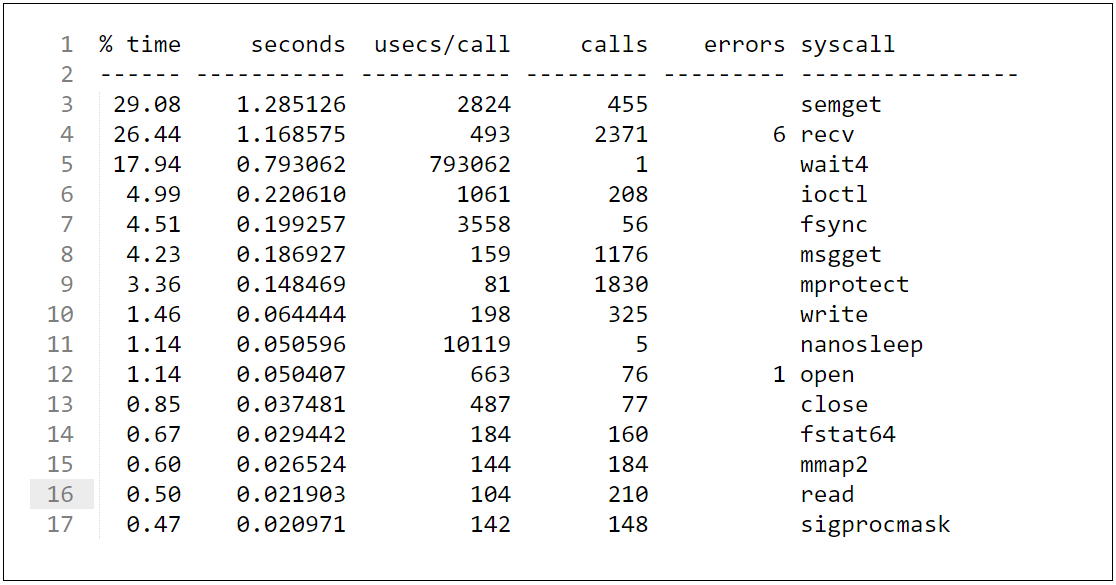
\includegraphics[width=1\textwidth]{single-strace-log.png}
    \caption{System call trace of an application}
    \label{fig:single-strace-log}
\end{figure}

\section{Evaluating our model}
\label{sec:syscalleval}

We wrote a java program linklink which further processes these files and assess our model.

The program divides the trace files into two datasets, training and validation. 50 malwares and 50 non-malware traces are chosen randomly and put in the validation dataset. The rest of the traces are used to train the classifier. The details of the training and classification steps are described in the following sub-sections.

\subsection{Training}
\label{subsec:syscallevaltrain}

The program aggregates all the traces in the training dataset and produce two relation matrices $M_{mal}$ and $M_{nmal}$. $M_{mal}$ and $M_{nmal}$ are defined in the previous chapter. A sample relation matrix is shown in figure~\ref{fig:sample-matrix}.

\begin{figure}[h!]
    \centering
    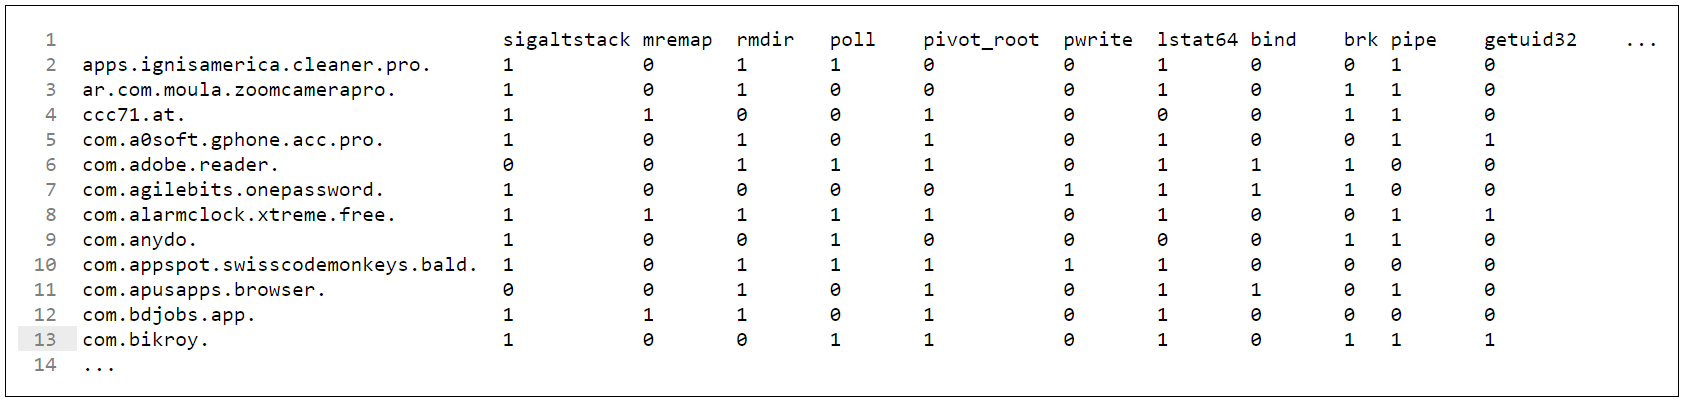
\includegraphics[width=1\textwidth]{relation_matrix.png}
    \caption{A sample relation matrix between syscalls and apps}
    \label{fig:sample-matrix}
\end{figure}

The two relation matrices are used to calculate the \textbf{Goodness rating}s of all syscalls.

\subsection{Classification}
\label{subsec:syscallevalclassify}
After \textbf{Goodness rating}s of all apps have been calculated, our model is ready to calssify an unlabeled app as malware or non-malware, given its system call trace. The same program calculates Goodness raings of all applications in the validation dataset, using the equation given in section~\ref{sec:syscalltheoryclassify}. If the Goodness rating of an app is lower than a \textbf{Threshold ($T$)}, our model/program flags the app as a malware, otherwise the app is considered to be non-malware.\\

We discuss the results achieved from our model in the following chapter.

\chapter{Results}
\label{chap:results}

We tried different thresholds and for each threshold, we ran our classifier for all validation apps and calculated different metrics like \textbf{Accuracy} ($ACC$), \textbf{True Positive Rate} ($TPR$), \textbf{Specificity} ($SPC$), \textbf{Positive Predictive Value} ($PPV$) and \textbf{F-measure} ($F$). We started from a threshold value of $-200$ and ended with $1500$, with step $10$. So the classifier was run a total of 171 times (each time with all validation apps).\\

Ideally, the \textbf{Threshold ($T$)} should be zero, but our experiment showed better accuracy for other values. To be exact, the best accuracy (87\%) is achieved when we use a threshold value between 300-340.\\

The \textbf{Threshold ($T$)} vs \textbf{Accuracy} ($ACC$) graph is shown in Figure~\ref{fig:thvsacc}.\\

\begin{figure}[h!]
    \centering
    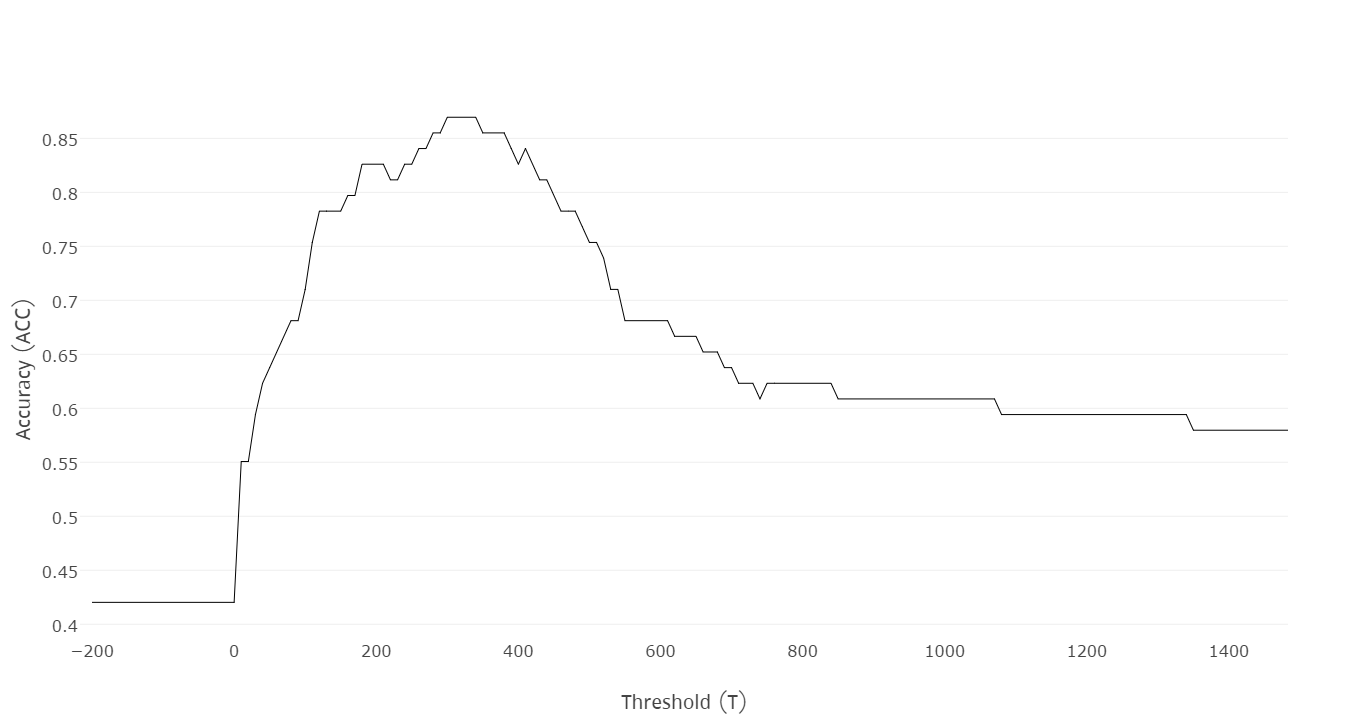
\includegraphics[width=1\textwidth]{thvsacc.png}
    \caption{\textbf{Threshold ($T$)} vs \textbf{Accuracy} ($ACC$) graph}
    \label{fig:thvsacc}
\end{figure}

The effect of threshold on other performance metrics of the classifier is shown in Figure ~\ref{fig:thvsppv} to ~\ref{fig:thvsfm}.
Figure~\ref{fig:thvsppv} shows $PPV = 87.8\%$ for $T = 320$.\\

\begin{figure}[h!]
    \centering
    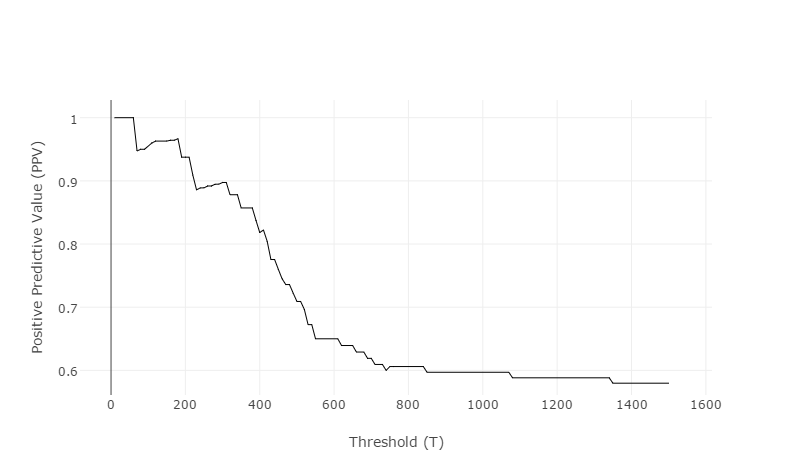
\includegraphics[width=1\textwidth]{thvsppv.png}
    \caption{\textbf{Threshold ($T$)} vs \textbf{Positive Predictive Value} ($PPV$) graph}
    \label{fig:thvsppv}
\end{figure}

Figure~\ref{fig:thvsspc} shows \textbf{Specificity}, $SPC = 82.7\%$ for $T = 320$.\\

\begin{figure}[h!]
    \centering
    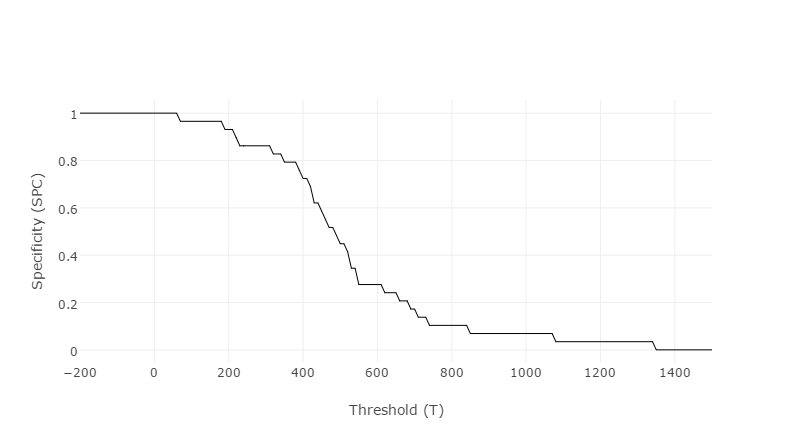
\includegraphics[width=1\textwidth]{thvsspc.png}
    \caption{\textbf{Threshold ($T$)} vs \textbf{Specificity} ($SPC$) graph}
    \label{fig:thvsspc}
\end{figure}

Figure~\ref{fig:thvstpr} shows \textbf{True Positive Rate}, $TPR = 90.1\%$ for $T = 320$.\\

\begin{figure}[h!]
    \centering
    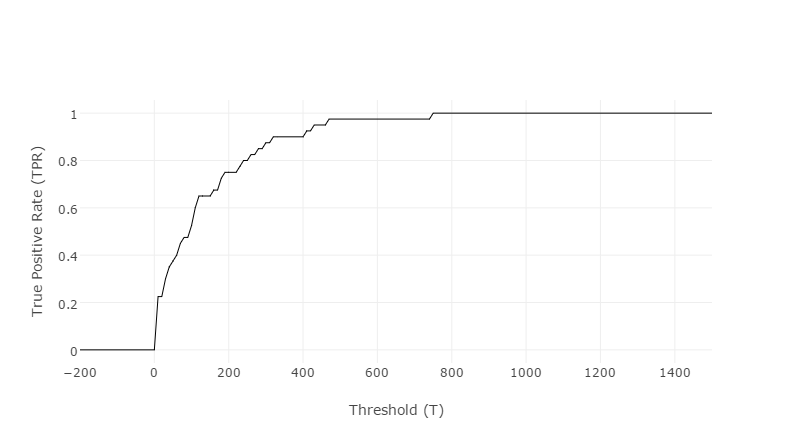
\includegraphics[width=1\textwidth]{thvstpr.png}
    \caption{\textbf{Threshold ($T$)} vs \textbf{True Positive Rate} ($TPR$) graph}
    \label{fig:thvstpr}
\end{figure}

And at last, Figure~\ref{fig:thvsfm} also shows a very good \textbf{F-measure} of $88.9$ for $T = 320$.\\

\begin{figure}[h!]
    \centering
    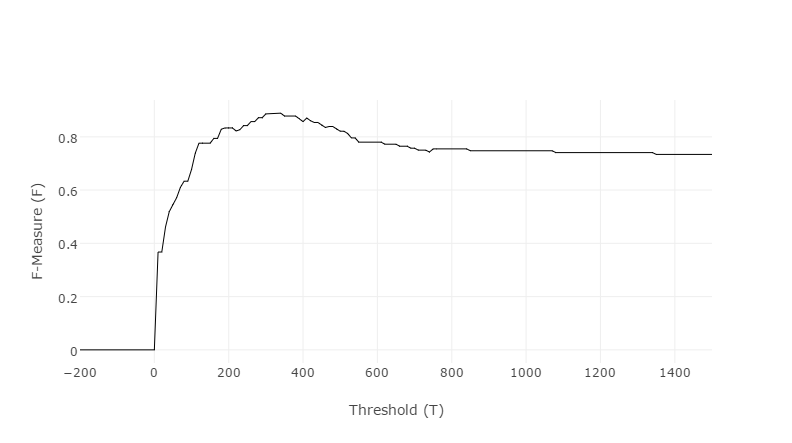
\includegraphics[width=1\textwidth]{thvsfm.png}
    \caption{\textbf{Threshold ($T$)} vs \textbf{F-measure} ($F$) graph}
    \label{fig:thvsfm}
\end{figure}

According to all these performance metrics, $320$ seems to be a very plausible value as \textbf{Threshold}, ($T$) for our model. The \textbf{Confusion Matrix} [explanation] of our model which uses $T = 320$ is shown in Figure~\ref{fig:confmatrix}.\\

\begin{figure}[h!]
    \centering
    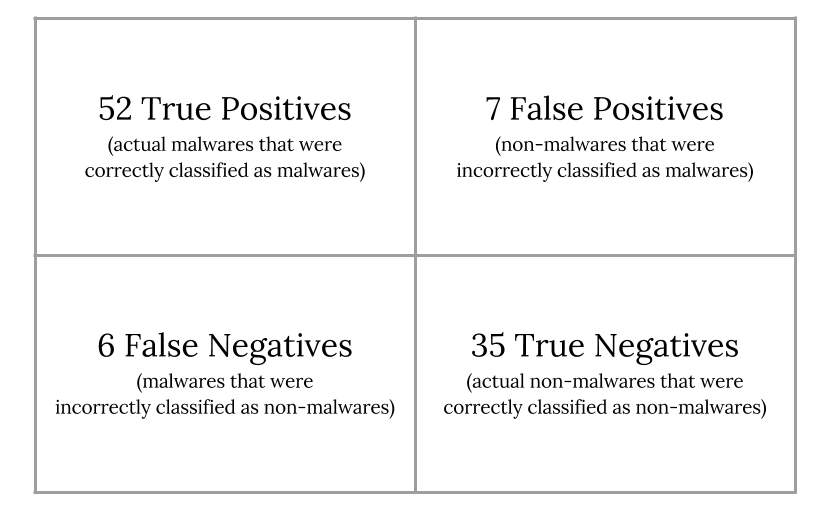
\includegraphics[width=0.75\textwidth]{confmatrix.png}
    \caption{\textbf{Confusion Matrix} with $T = 320$}
    \label{fig:confmatrix}
\end{figure}

Although we used widely variying types of malware and non-malware application samples in training and validation of our data, it is very difficult to amass a set of malware and non-malware apps that correctly emulates the distribution of all malwares in the wild and all non-malware apps in Google Play Store. So our experimentally achieved value for parameters like threshold might not be a good choice in all cases. But if we can feed the classifier a decent representative set of malwares and non-malwares, it should produce very usable results.

